\section{Verification, reproducibility and remaining scope}
\label{sec:validation}

\subsection{Exact algebraic certificates}

The program \code{code/verify_order_defect.py} builds the linear map
$X\mapsto(\sigma(g)X-X\rho(g))_g$ directly from generator matrices,
computes its integer Smith normal form, and takes the valuations at the
specified coefficient prime. This checks the claimed $p$-adic invariant
factors with exact arithmetic. It also computes the image-order Smith
exponents from the displayed bases. The recorded run contains 27 cases
across the sharp exponent family, the sharp length family and the
scalar-twist profile, and five complete finite-level kernel enumerations.
Every check passed. Full matrices, exponents and counts are in
\code{data/order_defect_certificates.json}.

For example, at $d=2$, $p=3$, $a=3$, $e=2$, the sharp length family has
profile $(2,2,2,3)$. The lengths at precisions $n=1,2,3,4$ are
$4,8,9,9$, respectively, exactly
$\min(n,3)+3\min(n,2)$. In the sharp exponent family with the same
$a,e$, the profile is $(0,0,0,5)$, so a cyclic congruence direction lasts
to depth $5$ even though the trace depth is $3$. These examples check
different assertions: the worst possible total length and the longest
possible individual direction need not occur in the same example.

\begin{figure}[htbp]
 \centering
 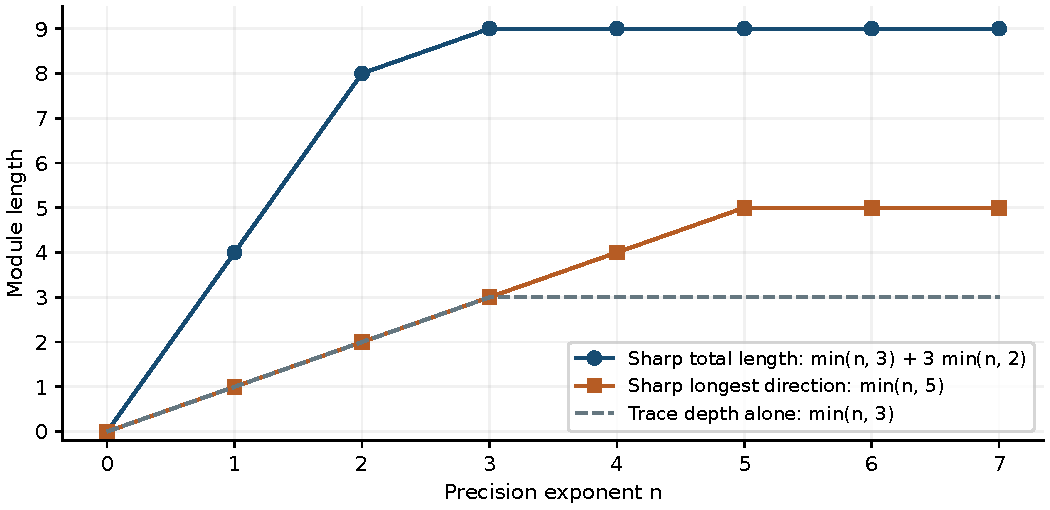
\includegraphics[width=0.94\textwidth]{figures/congruence_lengths.pdf}
 \caption{Exact finite-precision lengths in two extremal rank-two
 families with $a=3$, $e=2$. The first saturates the universal total
 bound; the second saturates the largest-exponent bound $a+e$. The
 curves are values of the proved formulas, not fitted measurements.}
 \label{fig:congruence}
\end{figure}

\subsection{Independent analytic checks}

The program \code{code/verify_grid_projection.py} constructs the averaging
coefficients in two ways: repeated integer convolution and a separate
inclusion--exclusion formula. The run checks 3,318 coefficients exactly,
including positivity, total mass, symmetry and the first two moments.
It also compares the polynomial and exponential multiplier formulas in
160 complex cases at 85-digit working precision and examines 42,000
points of the contraction envelope. The maximum recorded relative
multiplier discrepancy is below $7.5\cdot10^{-85}$.
These numerical comparisons are diagnostics; the inequalities for all
frequencies are proved in Lemma~\ref{grid:lem:contraction}.

\begin{figure}[htbp]
 \centering
 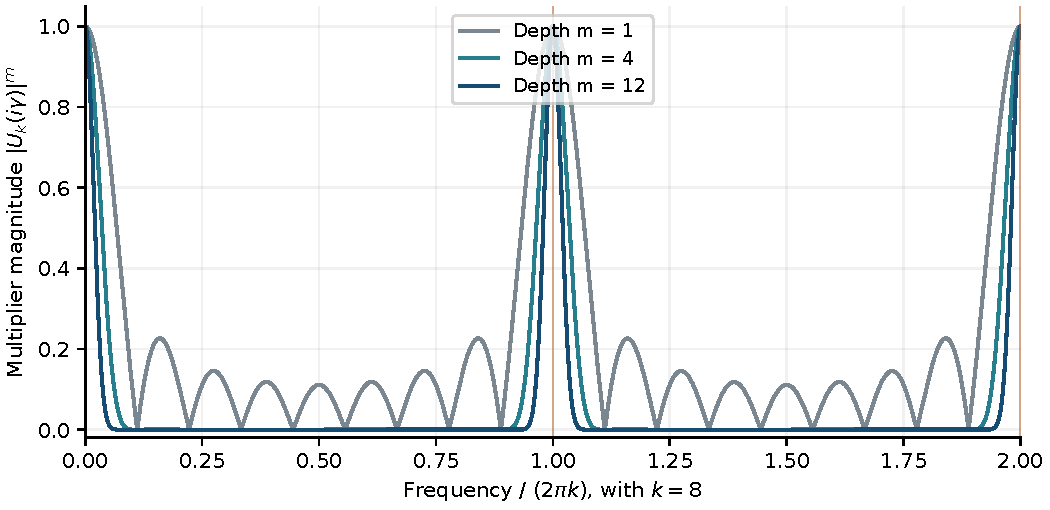
\includegraphics[width=0.94\textwidth]{figures/filter_aliases.pdf}
 \caption{The exact multiplier magnitude $|U_8(i\gamma)|^m$ at three
 depths. Increasing depth damps frequencies away from the lattice
 $2\pi k\mathbb Z$, while every alias remains equal to one. The local
 zero count, not a false uniform damping claim, controls those peaks
 in Theorem~\ref{grid:thm:abstract}.}
 \label{fig:aliases}
\end{figure}

For a direct prime-side illustration the script enumerates 37,128 primes
and 37,308 prime powers through $442{,}413$. It evaluates the identity-class
weight modulo $4$ and the weight $\chi_0+\Re\chi$ for the quartic
character modulo $5$ with $\chi(2)=i$. No zero table or $L$-value routine
is used. With $k=32$, $m=12$, and $t=0$, the values of the normalized
central-order statistic are approximately $0.1862897638670$ and
$0.1727260777212$. These small-depth demonstrations are not certified
central-order determinations and are not asserted to satisfy the
theorem's sufficient rounding threshold. They illustrate the direct
arithmetic computation, including its still-visible decaying remainder.
The complete results are in \code{data/grid_projection_results.json}.

\subsection{What the certificates establish}

The general algebraic theorem is established by its proof, not by a
finite search. The exact computations test its examples and the
implementation of their relation maps. The general analytic theorem is
established by its Fourier estimate and the explicit formula, not by
sampling frequencies. In particular no finite zero computation is used
to infer simplicity, central nonvanishing, or a bound uniform in all
conductors.

Both proofs received a separate internal mathematical review during
preparation. This is distinct from a proof-assistant check or external
peer review. No Lean executable was available in this research
environment, and no new Lean proof is claimed. The file
\code{formalization_outline.md} gives the definitions, intermediate
lemmas and dependency order for a future formalization without embedding
unproved assertions in an apparently completed Lean file.

\subsection{Reproduction and useful next questions}

The archive is self-contained for the new proofs and computations. A
standard LaTeX distribution builds \code{report.tex}; the Python scripts
need SymPy, mpmath, NumPy and Matplotlib, with exact instructions in
\code{README.md}. Upstream repositories are pinned and linked rather
than copied. The provenance files record inspected source hashes,
nearby results and the distinction between classical ingredients and
the proposed new conclusions.

For the algebraic theorem, a finer bound using the entire elementary
divisor profile of each image order could improve specific examples
without changing the sharp universal coefficient. One must still
verify the separate local and automorphic hypotheses before using the
new correction in an enlarged Selmer construction.
For the analytic theorem, worthwhile further work is to instantiate
effective gap and remainder constants for a chosen conductor and to
optimize the finite filter for those constants. The present rate holds
for each fixed family. The synthetic lower bound explains its lattice
alias term but does not establish optimality among all irregular
sampling schedules or among actual Dirichlet zero spectra.
